\newenvironment{styleColorfulGridAccenti}{}{}
\newcommand{\textstyleBookTitle}[1]{#1}
\newcommand{\textstyleSubtleEmphasis}[1]{#1}
\newcommand{\textstylehps}[1]{#1} 
\newcommand{\textstyleatn}[1]{#1}
\newcommand{\biberror}[1]{\color{red}\bfseries #1}


\newcommand{\qu}[1]{>>#1<<} % >> <<
\newcommand{\quein}[1]{>#1<} %einfache > <
\newcommand{\sem}[1]{\emph{#1}}  

% Thanks to Martin Scharrer
\newcolumntype{R}[2]{%
	>{\adjustbox{angle=#1,lap=\width-(#2)}\bgroup}%
	l%
	<{\egroup}%
}
\newcommand*\rot{\multicolumn{1}{R{90}{1em}}}

% Dcolumn
\newcolumntype{d}[1]{D{.}{.}{#1}}
 
\usetikzlibrary{fit}
\usetikzlibrary{positioning}
\usetikzlibrary{backgrounds}


% tikz

\newbox\MooringRope
\sbox\MooringRope{%
\begin{tikzpicture}
	\clip 	[rounded corners=.5cm] (0,0) rectangle (2,2);
	\node 	[minimum size=2cm, inner sep=0pt,outer sep=0pt,clip] (image) at (1,1) {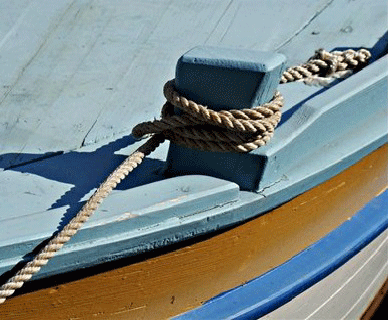
\includegraphics[height=2cm]{illustrations/skevin_fig3_mankul}};
	\draw 	[rounded corners=.5cm]
			([shift={(0.5\pgflinewidth,0.5\pgflinewidth)}]0,0) rectangle
			([shift={(-0.5\pgflinewidth,-0.5\pgflinewidth)}]2,2);
\end{tikzpicture}}

\newbox\FishingTool
\sbox\FishingTool{%
\begin{tikzpicture}
	\clip 	[rounded corners=.5cm] (0,0) rectangle (2,2);
	\node 	[minimum size=2cm, inner sep=0pt,outer sep=0pt,clip] (image) at (1,1) {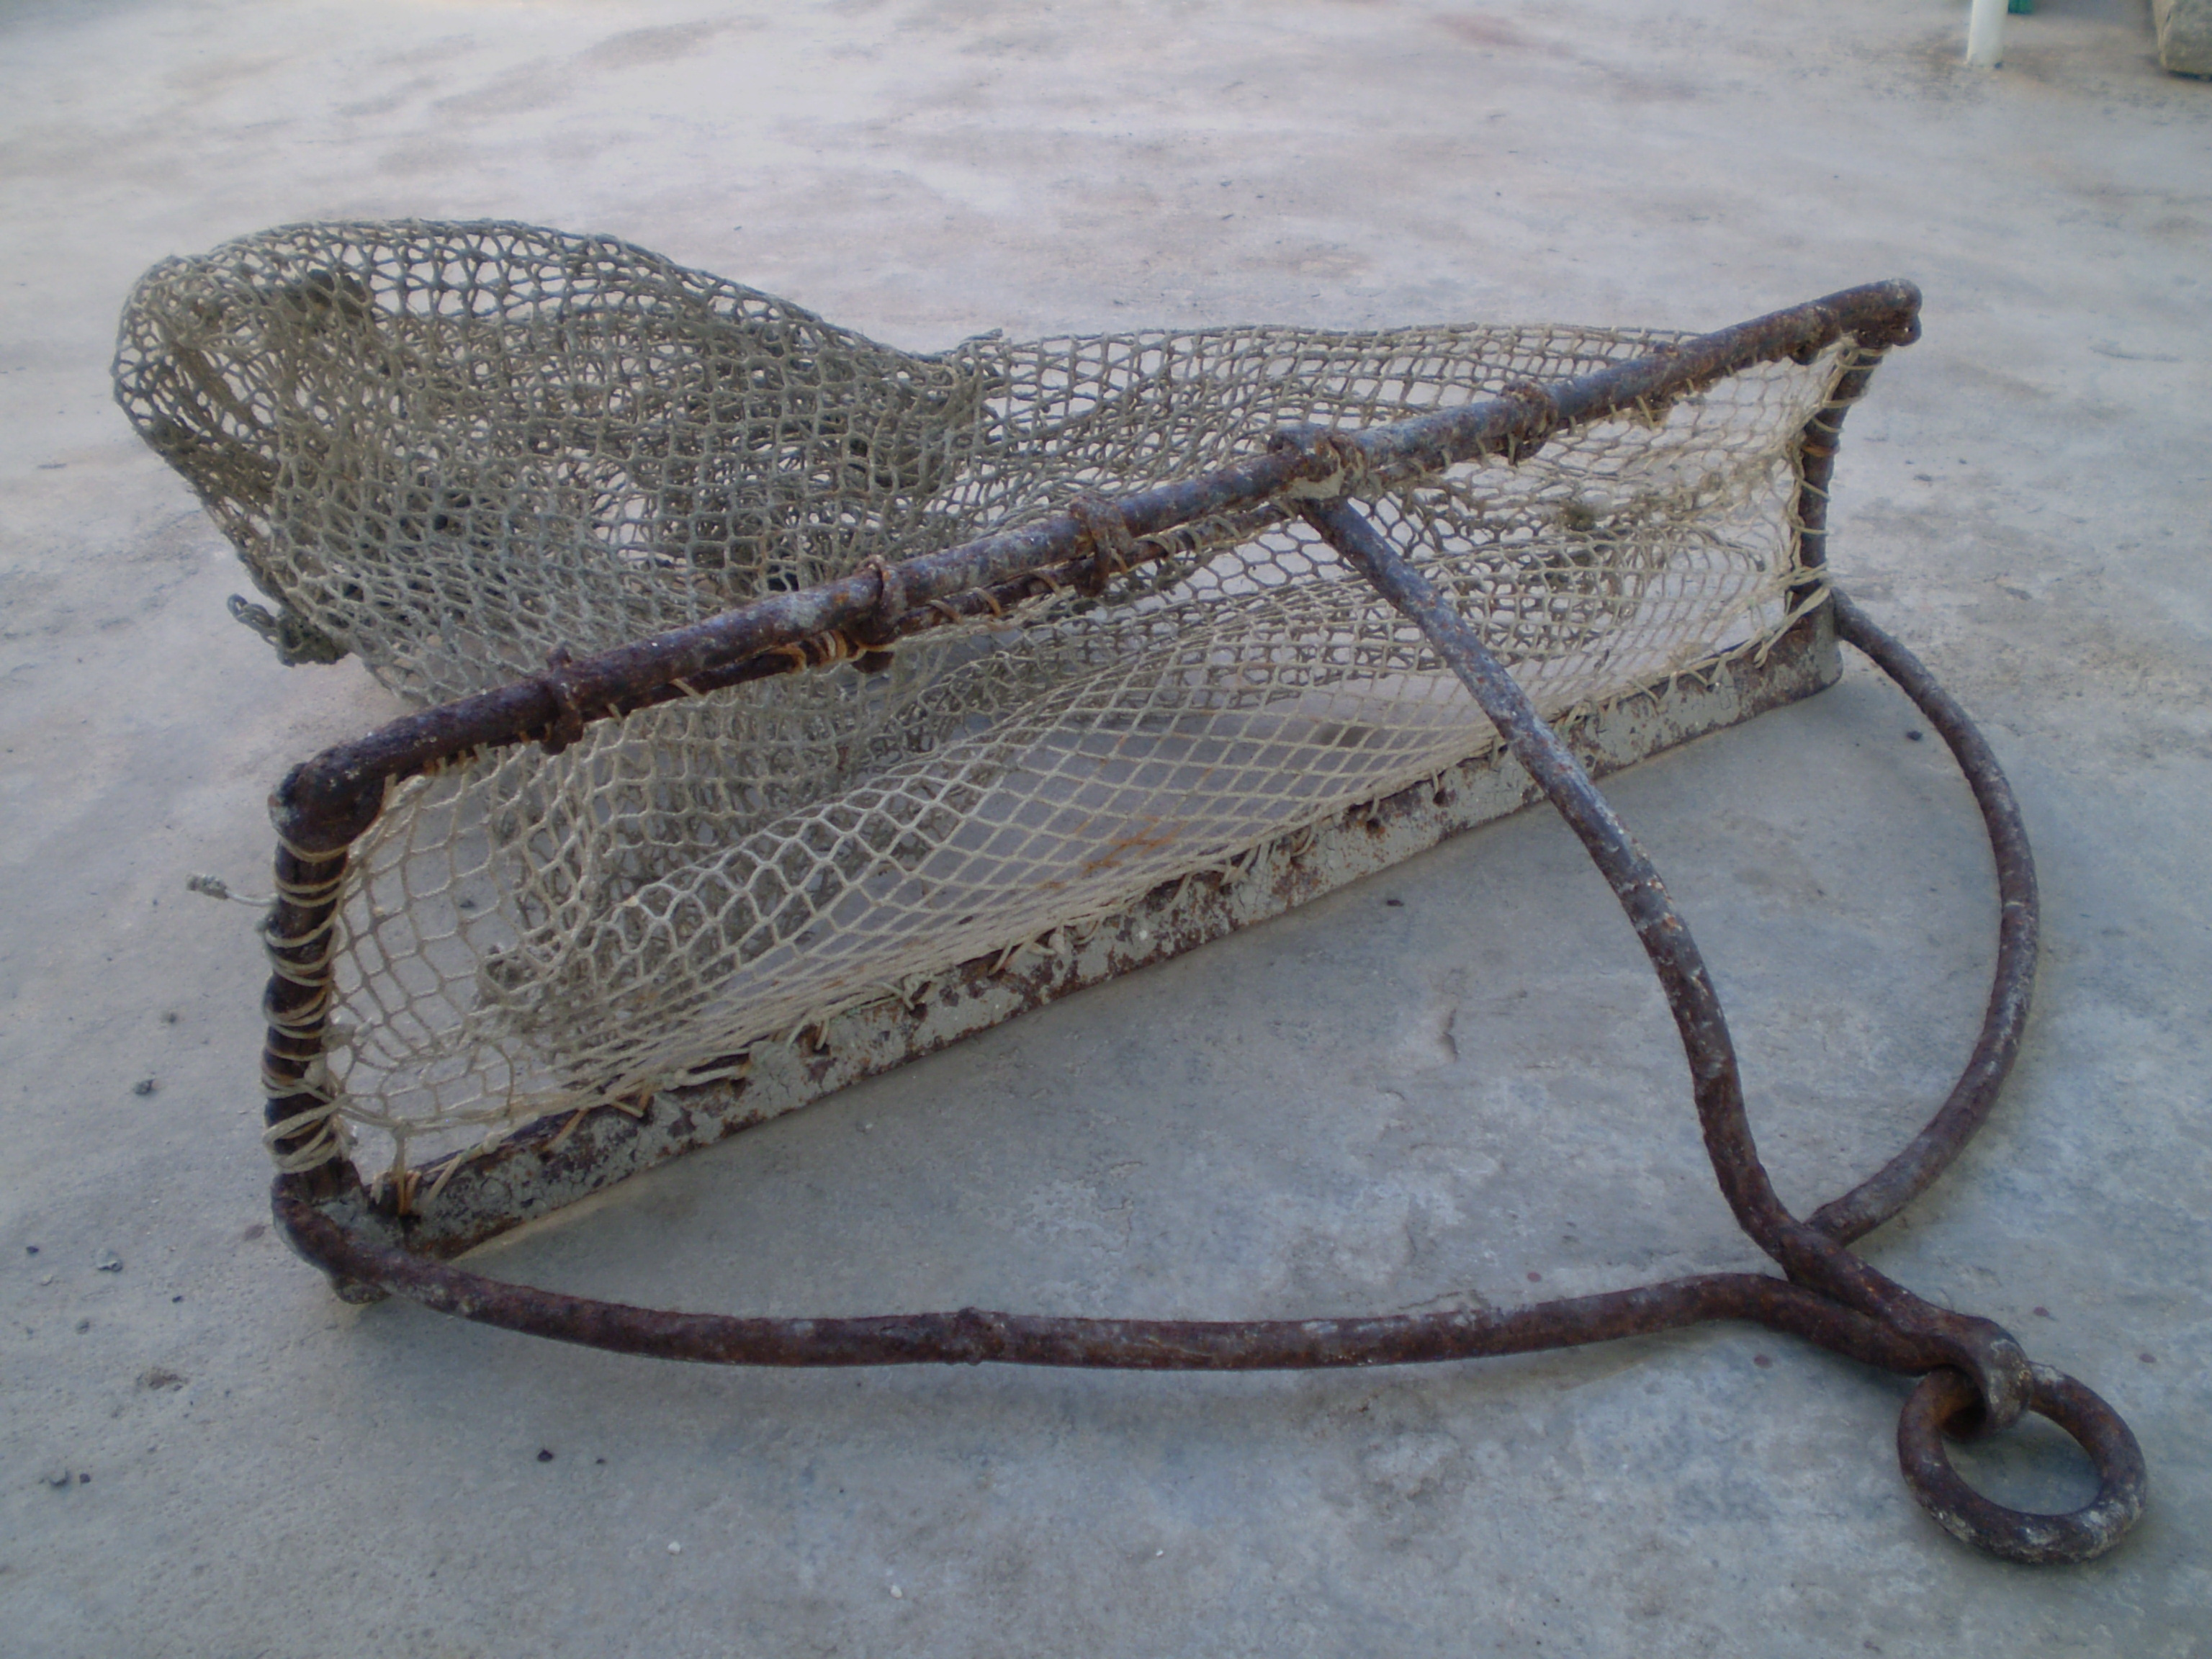
\includegraphics[height=2cm]{illustrations/skevin_fig4_brganja}};
	\draw 	[rounded corners=.5cm]
			([shift={(0.5\pgflinewidth,0.5\pgflinewidth)}]0,0) rectangle
			([shift={(-0.5\pgflinewidth,-0.5\pgflinewidth)}]2,2);
\end{tikzpicture}}

\newbox\OtherFishingTool
\sbox\OtherFishingTool{%
\begin{tikzpicture}
	\clip 	[rounded corners=.5cm] (0,0) rectangle (2,2);
	\node 	[minimum size=2cm, inner sep=0pt,outer sep=0pt,clip] (image) at (1,1) {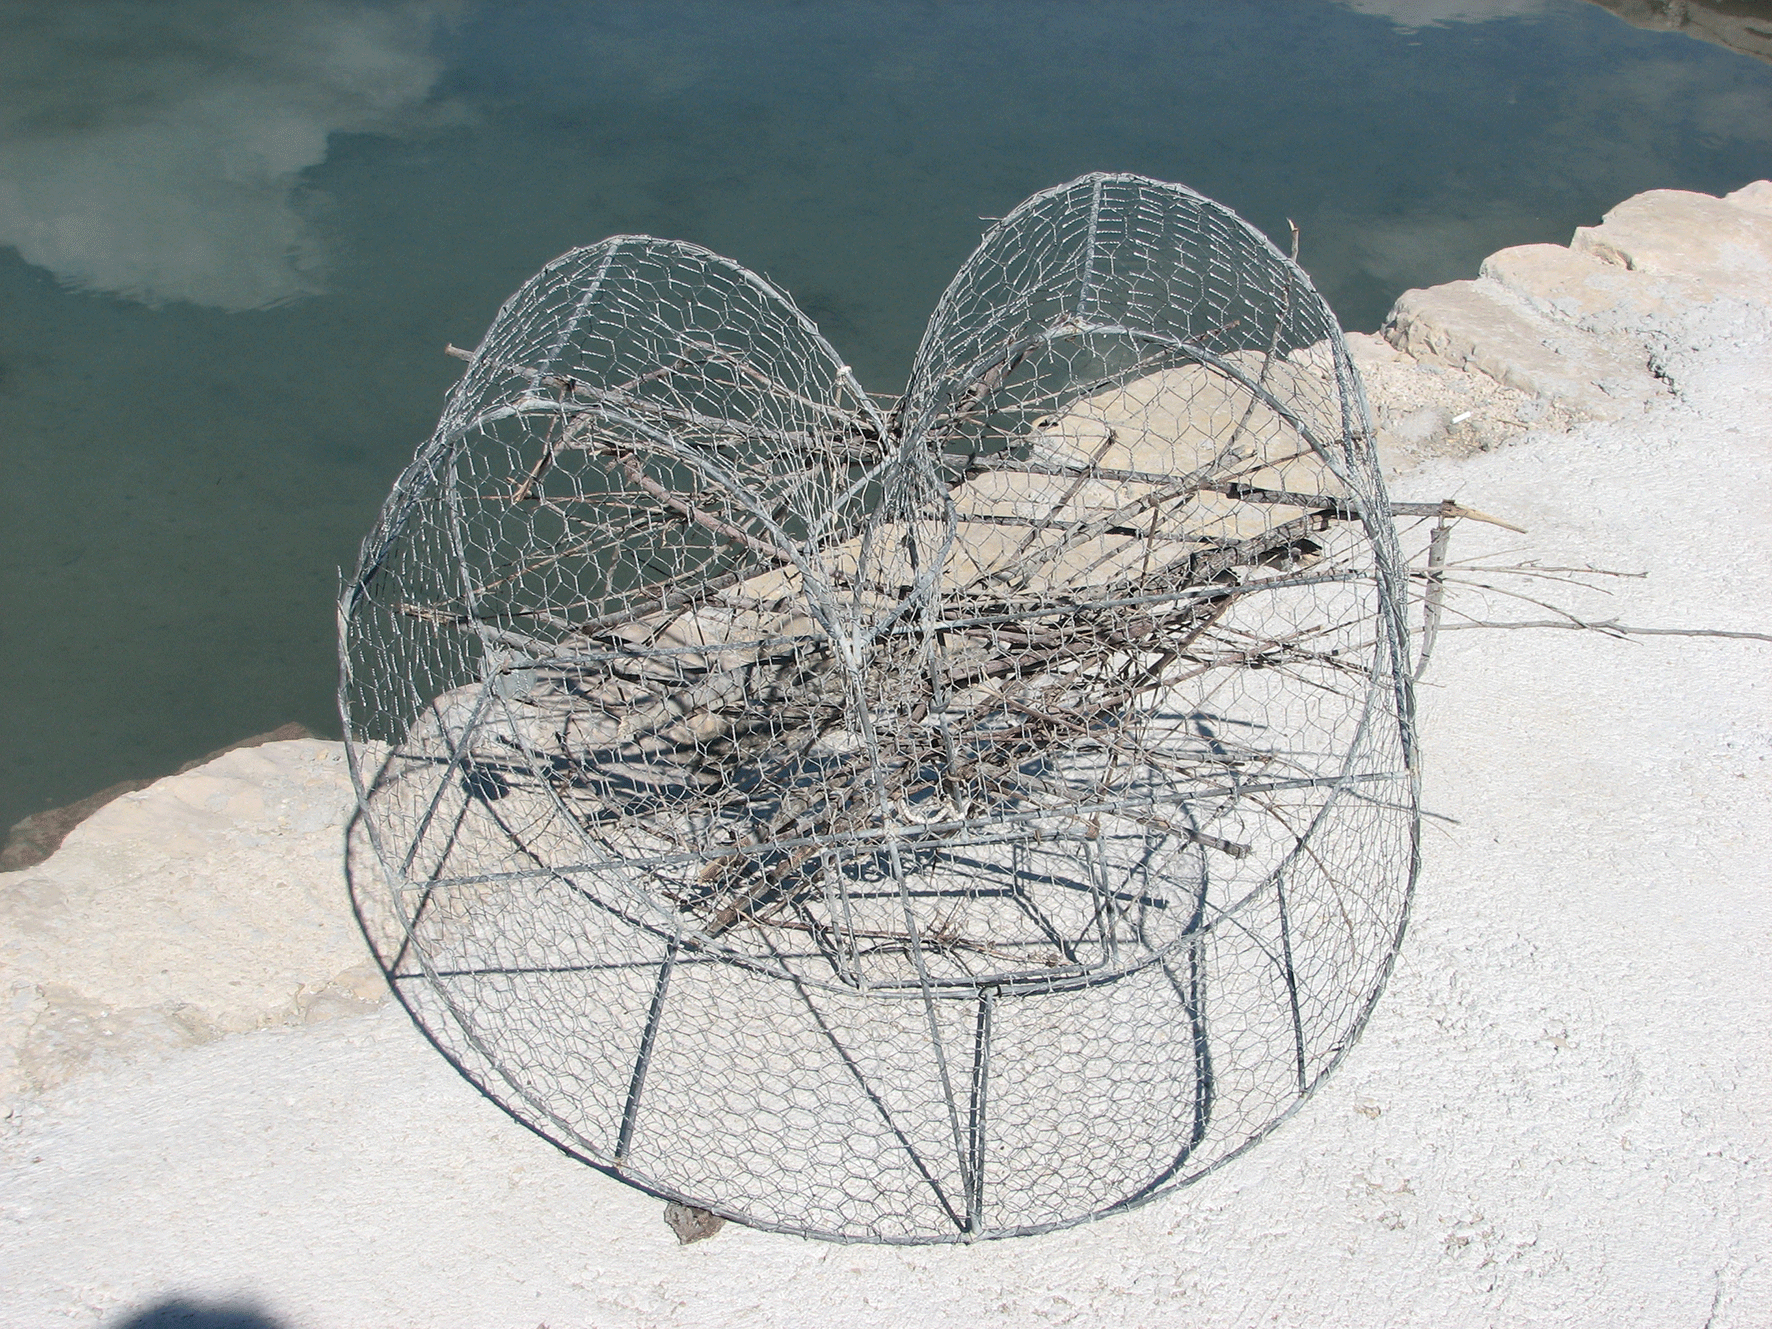
\includegraphics[height=2cm]{illustrations/skevin_fig4_vrsa}};
	\draw 	[rounded corners=.5cm]
			([shift={(0.5\pgflinewidth,0.5\pgflinewidth)}]0,0) rectangle
			([shift={(-0.5\pgflinewidth,-0.5\pgflinewidth)}]2,2);
\end{tikzpicture}}

\newcommand*{\MankulOldSpeakers}[1]{%
\begin{tikzpicture}
	[
		scale=#1,
		every node/.style={
			anchor=base,
			minimum height=\ht\MooringRope,
			text centered,
			fill=white,
			transform shape
		}
	]
	\node	[align=center,draw,rounded corners=.25cm] (trans) at (3,3) {`A thick wooden post\\around which a mooring\\rope is tied.'};
	\node	[below left = 2.5cm of trans,draw] (native) at (2,0) {\itshape\textbf{manku(l)} m.};
	\node	[below right = 2.5cm of trans,inner sep=0pt,outer sep=0pt] (image) at (4,0) {\usebox\MooringRope};
	\begin{scope}[on background layer]
		\draw	(native.west) to (trans.north);
		\draw	(image.east) to (trans.north);
		\draw	(native.west) to (image.east);
	\end{scope}
\end{tikzpicture}}

\newcommand*{\MankulYoungAdults}[1]{%
\begin{tikzpicture}
	[
		scale=#1,
		every node/.style={
			anchor=base,
			minimum height=\ht\MooringRope,
			text centered,
			fill=white,
			transform shape
		}
	]
	\node	[align=center,draw,minimum width=4cm,rounded corners=.25cm] (trans) at (3,3) {`Something on a\\boat?'};
	\node	[below left = 2.5cm of trans,draw] (native) at (2,0) {\itshape\textbf{manku(l)} m.};
	\node	[below right = 2.5cm of trans,inner sep=0pt,outer sep=0pt] (image) at (4,0) {\usebox\MooringRope};
	\node	[left = 0cm of image,draw] (unsure) {\bfseries ?};
	\begin{scope}[on background layer]
		\draw	(native.west) to (trans.north);
		\draw	(image.east) to (trans.north);
		\draw	(native.west) to (image.east);
	\end{scope}
\end{tikzpicture}}

\newcommand*{\BrganjaOldSpeakers}[1]{%
\begin{tikzpicture}
	[
		scale=#1,
		every node/.style={
			anchor=base,
			minimum height=\ht\FishingTool,
			text centered,
			fill=white,
			transform shape
		}
	]
	\node	[align=center,draw,rounded corners=.25cm] (trans) at (3,3) {`A type of a fishing tool\\used to collect different kinds\\of seashells by dragging it\\across the sea floor.'};
	\node	[below left = 2.5cm of trans,draw] (native) at (2,0) {\itshape\textbf{brganja} f.};
	\node	[below right = 2.5cm of trans,inner sep=0pt,outer sep=0pt] (image) at (4,0) {\usebox\FishingTool};
	\begin{scope}[on background layer]
		\draw	(native.west) to (trans.north);
		\draw	(image.east) to (trans.north);
		\draw	(native.west) to (image.east);
	\end{scope}
\end{tikzpicture}}

\newcommand*{\BrganjaYoungAdults}[1]{%
\begin{tikzpicture}
	[
		scale=#1,
		every node/.style={
			anchor=base,
			minimum height=\ht\OtherFishingTool,
			text centered,
			fill=white,
			transform shape
		}
	]
	\node	[align=center,draw,rounded corners=.25cm] (trans) at (3,3) {`A net used for\\collecting seashells.'};
	\node	[below left = 2.5cm of trans,draw] (native) at (2,0) {\itshape\textbf{brganja} f.};
	\node	[below right = 2.5cm of trans,inner sep=0pt,outer sep=0pt] (image) at (4,0) {\usebox\OtherFishingTool};
	\node 	[right = 0em of image,draw,yshift=-10pt] (unsure) {\bfseries ?};
	\node	[left = 0em of image,inner sep=0pt,outer sep=0pt,yshift=-10pt] (FishingTool) {\usebox\FishingTool};
	\begin{scope}[on background layer]
		\draw	(native.west) to (trans.north);
		\draw	(image.east) to (trans.north);
		\draw	(native.west) to (image.east);
	\end{scope}
\end{tikzpicture}}

\newcommand*{\BrganjaYoungAdultsSemanticExtension}[1]{%
\begin{tikzpicture}
	[
		scale=#1,
		every node/.style={
			anchor=base,
			minimum height=\ht\OtherFishingTool,
			text centered,
			fill=white,
			transform shape
		}
	]
	\node	[align=center,draw,rounded corners=.25cm] (trans) at (3,3) {`A net used for\\collecting seashells.'};
	\node	[right = 1.5cm of trans,align=center,draw,rounded corners=.25cm] (SemanticExtension) {`A summer festivity\\celebrated every first\\Sunday in August.'};
	\node	[below left = 2.5cm of trans,draw] (native) at (2,0) {\itshape\textbf{brganja} f.};
	\node	[below right = 2.5cm of trans,inner sep=0pt,outer sep=0pt] (image) at (4,0) {\usebox\OtherFishingTool};
	\node 	[right = 0em of image,draw,yshift=-10pt] (unsure) {\bfseries ?};
	\node	[left = 0em of image,inner sep=0pt,outer sep=0pt,yshift=-10pt] (FishingTool) {\usebox\FishingTool};
	\draw[vecArrowOlive] (trans) to (SemanticExtension);
	\draw[vecOpenArrowRed] (trans) to (SemanticExtension);
	\draw[innerOlive] (trans) to (SemanticExtension);
	\begin{scope}[on background layer]
		\draw	(native.west) to (trans.north);
		\draw	(image.east) to (trans.north);
		\draw	(native.west) to (image.east);
	\end{scope}
\end{tikzpicture}}

\newcommand*{\DumplirOldSpeakers}[1]{%
\begin{tikzpicture}
	[
		scale=#1,
		every node/.style={
			anchor=base,
			minimum height=\ht\OtherFishingTool,
			text centered,
			fill=white,
			transform shape
		}
	]
	\node	[align=center,draw,rounded corners=.25cm] (trans) at (3,3) {`A type of a candle\\carried during a\\funeral.'};
	\node	[below left = 2.5cm of trans,draw] (native) at (2,0) {\itshape\textbf{dumplir} m.};
	\node	[below right = 2.5cm of trans,inner sep=0pt,outer sep=0pt,rounded corners=.25cm,minimum width=\wd\FishingTool,draw] (image) at (4,0) {\bfseries ?};
	\begin{scope}[on background layer]
		\draw	(native.west) to (trans.north);
		\draw	(image.east) to (trans.north);
		\draw	(native.west) to (image.east);
	\end{scope}
\end{tikzpicture}}
\newcommand*{\DumplirYoungAdults}[1]{%
\begin{tikzpicture}
	[
		scale=#1,
		every node/.style={
			anchor=base,
			minimum height=\ht\OtherFishingTool,
			text centered,
			fill=white,
			transform shape
		}
	]
	\node	[align=center,draw,rounded corners=.25cm] (trans) at (3,3) {`A type of a candle\\carried during a\\funeral.'};
	\node	[below left = 2.5cm of trans,draw] (native) at (2,0) {\itshape\textbf{dumplir} m.};
	\node	[below right = 2.5cm of trans,inner sep=0pt,outer sep=0pt,rounded corners=.25cm,minimum width=\wd\FishingTool,draw] (image) at (4,0) {\bfseries ?};
	\draw	[semithick] ($(trans.south west)+(0.25,0.25)$) to ($(trans.north east)-(0.25,0.25)$);
	\begin{scope}[on background layer]
		\draw	(native.west) to (trans.north);
		\draw	(image.east) to (trans.north);
		\draw	(native.west) to (image.east);
	\end{scope}
\end{tikzpicture}}
\newcommand*{\DumplirLossOfVariant}[1]{%
\begin{tikzpicture}
	[
		scale=#1,
		every node/.style={
			anchor=base,
			minimum height=\ht\OtherFishingTool,
			text centered,
			fill=white,
			transform shape
		}
	]
	\node	[align=center,draw,rounded corners=.25cm] (trans) at (3,3) {`A type of a candle\\carried during a\\funeral.'};
	\node	[below left = 2.5cm of trans,draw] (native) at (2,0) {\itshape\textbf{dumplir} m.};
	\node	[below right = 2.5cm of trans,inner sep=0pt,outer sep=0pt,rounded corners=.25cm,minimum width=\wd\FishingTool,draw] (image) at (4,0) {\bfseries ?};
	\draw	[semithick] ($(trans.south west)+(0.25,0.25)$) to ($(trans.north east)-(0.25,0.25)$);
	\draw	[semithick] (native.south west) to (native.north east);
	\begin{scope}[on background layer]
		\draw	(native.west) to (trans.north);
		\draw	(image.east) to (trans.north);
		\draw	(native.west) to (image.east);
	\end{scope}
\end{tikzpicture}}
